\section{Podzadanie E}
\subsection{Analiza danych}
\subsubsection{Format danych}

Format danych w tym podzadaniu jest wzbogacony o dodatkowe atrybuty dla znaczników XML: ,,RelQuestion'', ,,RelAnswer'' oraz ,,RelComment''. Umożliwia to pobranie większej liczby miar statystycznych niż w poprzednich przypadkach.

Element \emph{,,RelQuestion''} zawiera dodatkowe pola tj.: \emph{liczba punktów} czy \emph{liczba wyświetleń}. Są one wykorzystane przy sprawdzaniu miar statystycznych. Struktura tego elementu przedstawia się następująco:

\begin{lstlisting}[language=XML,breaklines,label={lst:subtask_e_rel_question},caption={Przykład elementu ,,RelQuestion''.}]
<RelQuestion RELQ_CATEGORY="cooking" RELQ_DATE="2015-09-28 12:36:51" RELQ_ID="236203783777_R223248892008" RELQ_RANKING_ORDER="1" RELQ_RELEVANCE2ORGQ="Irrelevant" RELQ_SCORE="1" RELQ_TAGS="indian-cuisine, texture" RELQ_USERID="39650" RELQ_USERNAME="" RELQ_VIEWCOUNT="82">
  <RelQSubject>
    Remedy for Dry Chicken Yakhni pulao ?
  </RelQSubject>
  <RelQBody>
    My question is that today I prepared Chicken Yakhni Pulao,it tasted good but it is very dry, i mean the youghurt and the masala got absorbed in the rice very much. And i have made lots of it, it is also fully cooked. So does anyone know how should i make the fully cooked pulao little juicy ? As it is difficult to eat the dry pulao(I may require another curry with it)
  </RelQBody>
</RelQuestion>
\end{lstlisting}

Element \emph{,,RelAnswer''} zawiera kilka dodatkowych atrybutów. Nie zostały one jednak wykrzystane w późniejszych eksperymentach. Struktura tego elementu przedstawia się następująco:

\begin{lstlisting}[language=XML,breaklines,label={lst:subtask_e_rel_answer},caption={Przykład elementu ,,RelAnswer''.}]
<RelAnswer RELA_ACCEPTED="0" RELA_DATE="2015-09-29 10:44:51" RELA_ID="236203783777_R223248892008_A506889689755" RELA_RELEVANCE2ORGQ="" RELA_RELEVANCE2RELQ="" RELA_SCORE="0" RELA_USERID="37725" RELA_USERNAME="">
  <RelAText>
    I recon it has formed like a cake after cooling. The best option you have is to take a big chunk of it in a microwaveable container (making sure that you are not breaking the rice grains) and sprinkling with some water. Then cover with a cling film and microwave for 3-4 minutes from cold. Your rice grains will separate because of the extra moisture from the sprinkled water and the Pulao will become slightly moist.   But yes, Pulao is a dry dish and needs to be eaten with a side like Raita or Salan.
  </RelAText>
</RelAnswer>
\end{lstlisting}

Podobnie jak poprzedni element, \emph{,,RelComment''} zawiera dodatkowe atrybuty, lecz nie zostały one wykorzystane. Struktura tego elementu wygląda w następujący sposób:

\begin{lstlisting}[language=XML,breaklines,label={lst:subtask_e_rel_comment},caption={Przykład elementu ,,RelComment''.}]
<RelComment RELC_DATE="2015-09-29 11:57:05" RELC_ID="236203783777_R223248892008_C246533537180" RELC_RELEVANCE2ORGQ="" RELC_RELEVANCE2RELQ="" RELC_SCORE="1" RELC_USERID="17272" RELC_USERNAME="">
  <RelCText>
    Are you trying to make it better next time, or salvage what you've already made?
  </RelCText>
</RelComment>
\end{lstlisting}

\subsubsection{Rozkład danych}
Podzadanie E miało na celu stwierdzenie czy dane pytanie jest duplikatem. Polega to na porównaniu przykładowego pytania z pytaniem istniejącym już na forum dyskusyjnym, które zawiera również wątek odpowiedzi oraz komentarzy. Zbiór danych pochodzi z forum ,,Stack Exchange - English Language''.
Oryginalny zbiór zawiera \emph{1035065 par pytań}, a jego rozkład danych przedstawia się następująco:

\begin{table}[H]
\caption{Rozkład klas w zbiorze uczącym.}
\label{se_train_set_unmodified}
    \begin{center}
        \begin{tabular}{ |c|c| } 
            \hline
            klasa & rozkład\\
            \hline
            PerfectMatch & 0,0468\% \\
            \hline
            Related & 0,7201\% \\
            \hline
            Irrelevant & 99,232\% \\
            \hline
        \end{tabular}
    \end{center}
\end{table}

W oryginalnym zbiorze danych przeważają przykłady oznaczone etykietą ,,Irrelevant''. Jest to problem, ponieważ nie pozwala to na poprawne wyuczenie sieci neuronowej. Rozwiązaniem tego problemu, może być dogenerowanie przykładów z etykietą ,,PerfectMatch''. Po modyfikacji zbioru danych, rozmiar zredukował się do \emph{30407 elementów}, a jego rozkład przedstawia się w taki sposób:

\begin{table}[H]
\caption{Rozkład klas w zmodyfikowanym zbiorze uczącym.}
\label{se_train_set_modified}
    \begin{center}
        \begin{tabular}{ |c|c| }
            \hline
            klasa & rozkład\\
            \hline
            PerfectMatch & 25,1619\% \\
            \hline
            Related & 24,5140\% \\
            \hline
            Irrelevant & 50,3239\% \\
            \hline
        \end{tabular}
    \end{center}
\end{table}

Udział klasy ,,PerfectMatch'' w zbiorze treningowym wynosi około 25\%, co~pozwala na dużo lepsze wyuczenie sieci neuronowej mimo zredukowanego rozmiaru zbioru uczącego.

Zadanie polega na stwierdzeniu czy pytanie jest duplikatem istniejącego już pytania, a wyłącznie etykieta ,,PerfectMatch'' odpowiada takiemu zdarzeniu, można więc zredukować zbiór danych do 2 klas: \emph{Duplicate} oraz \emph{Non-duplicate}. Rozkład klas przedstawia się wtedy następująco:

\begin{table}[H]
\caption{Rozkład zredukowanych klas w zbiorze uczącym.}
\label{se_train_set_reduced}
    \begin{center}
        \begin{tabular}{ |c|c| }
         \hline
         klasa & rozkład \\
         \hline
         Duplicate & 25,1619\% \\
         \hline
         Non-duplicate & 74,8381\% \\
         \hline
        \end{tabular}
    \end{center}
\end{table}

\subsection{Miary statystyczne}

Podobnie jak w przypadku poprzednich podzadań, pierwszą próbą rozwiązania tego problemu, było porównanie miar statystycznych dwóch tekstów w celu sprawdzenia podobieństwa między nimi. Istnieje jednak różnica między poprzednimi podzadaniami. W zbiorze danych dla podzadania E zostały dodane dodatkowe atrybuty. Problem z nierównością rozkładu klas nie dotyczy badań miar statystycznych, dlatego skorzystano z danych o rozkładzie przedstawionym w tablicy~ \ref{se_train_set_unmodified}. Wykonano jednak połączenie klas ,,Irrelevant'' oraz ,,Related'' w jedną klasę ,,Non-duplicate''. Etykieta ,,PerfectMatch'' została zamieniona na ,,Duplicate''.

\begin{figure}[H]
\centering
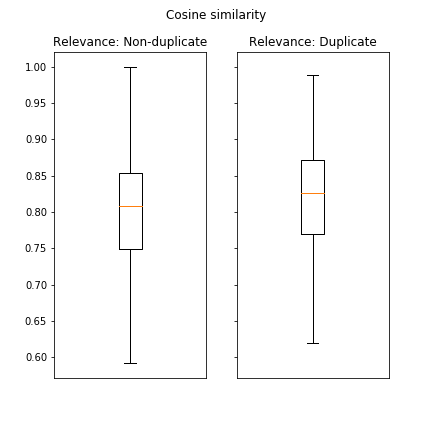
\includegraphics[scale=0.5]{e_en_train_cosine_similarity.png}
\caption{Zależność podobieństwa kosinusowego i klasy.}
\end{figure}

Porównując podobieństwa kosinusowe dla par tekstów oznaczonych etykietą ,,Duplicate'' oraz ,,Non-duplicate'' nie widać wyraźnej różnicy między wartościami mediany, pierwszego kwartylu ani trzeciego kwartylu. Dlatego na podstawie tej miary, nie jesteśmy w stanie stwierdzić podobieństwa między dwoma tekstami.

\begin{figure}[H]
\centering
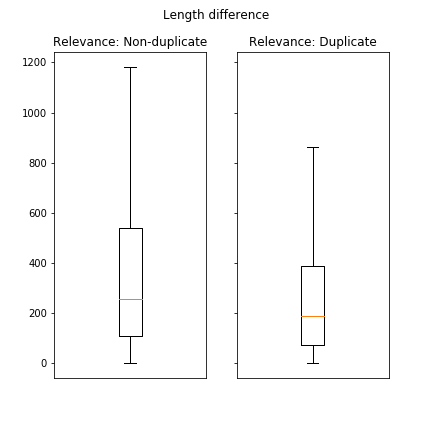
\includegraphics[scale=0.5]{e_en_train_length_difference.png}
\caption{Zależność różnicy długości i klasy.}
\end{figure}

Różnica długości dwóch tekstów, podobnie jak miara podobieństwa kosinusowego, nie jest w stanie sama określić podobieństwa między tymi tekstami.

\begin{figure}[H]
\centering
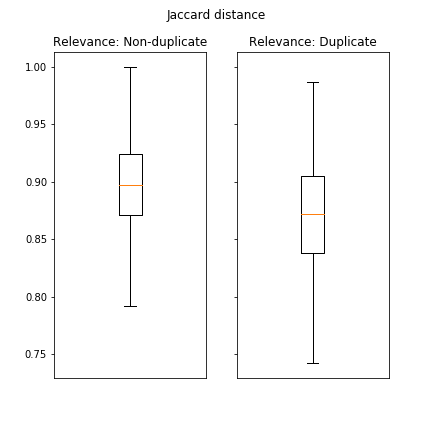
\includegraphics[scale=0.5]{e_en_train_jaccard_distance.png}
\caption{Zależność odległości Jaccarda i klasy}
\end{figure}

Dla większości par tekstów oznaczonych etykietą ,,Duplicate'', wartości znajdowały się w przedziale $\langle 0,85-0,92 \rangle$. Porównując to z wartościami dla par oznaczonych klasą ,,Non-duplicate'', nadal nie możemy stwierdzić które przypadki są duplikatami, a które nie.

Kolejne miary przedstawione na wykresach, są możliwe do wyznaczenia tylko w przypadku tego podzadania. Zbiór danych różni się atrybutami które są umieszczone w znacznikach XML. Wypróbowanych zostało 6 dodatkowych miar. Są to:

\begin{itemize}
\item liczba wyświetleń pytania powiązanego,
\item liczba punktów pytania powiązanego,
\item liczba odpowiedzi,
\item liczba komentarzy,
\item całkowita liczba głosów na odpowiedzi do pytania powiązanego,
\item liczba głosów na najlepszą odpowiedź do pytania powiązanego.
\end{itemize}

\begin{figure}[H]
    \begin{subfigure}{.5\textwidth}
        \label{fig:subtask_e_view_count}
        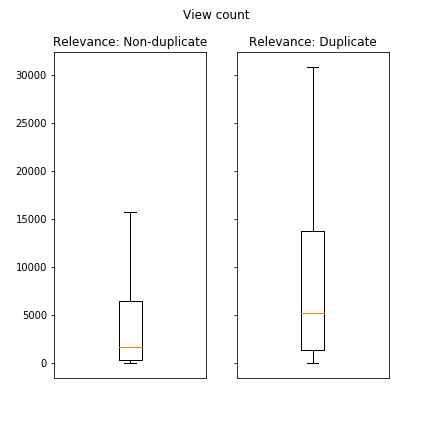
\includegraphics[width=\linewidth]{e_en_train_view_count.png}
        \caption{Liczba wyświetleń.}
    \end{subfigure}
    \begin{subfigure}{.5\textwidth}
        \label{fig:subtask_e_score}
        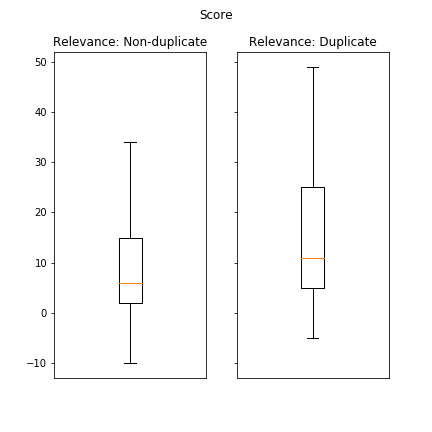
\includegraphics[width=\linewidth]{e_en_train_score.png}
        \caption{Liczba punktów.}
    \end{subfigure}
    \begin{subfigure}{.5\textwidth}
        \label{fig:subtask_e_no_of_answers}
        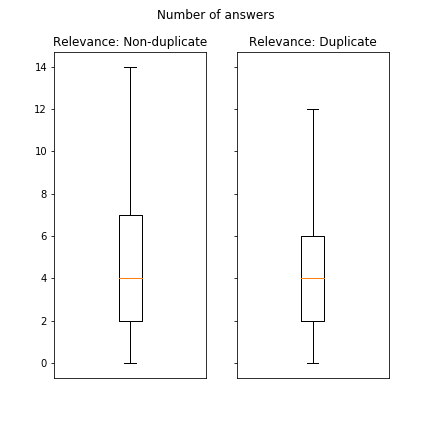
\includegraphics[width=\linewidth]{e_en_train_no_of_answers.png}
        \caption{Liczba odpowiedzi.}
    \end{subfigure}
    \begin{subfigure}{.5\textwidth}
        \label{fig:subtask_e_no_of_comments}
        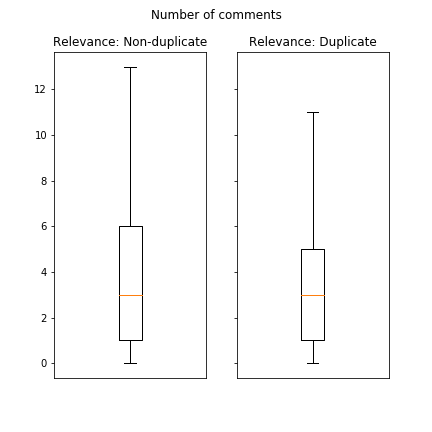
\includegraphics[width=\linewidth]{e_en_train_no_of_comments.png}
        \caption{Liczba komentarzy.}
    \end{subfigure}
    \begin{subfigure}{.5\textwidth}
        \label{fig:subtask_e_total_answer_upvotes}
        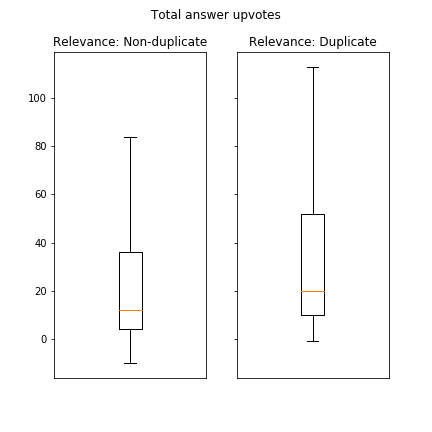
\includegraphics[width=\linewidth]{e_en_train_total_answer_upvotes.png}
        \caption{Liczba głosów na wszystkie odpowiedzi.}
    \end{subfigure}
    \begin{subfigure}{.5\textwidth}
        \label{fig:subtask_e_best_answer_upvotes}
        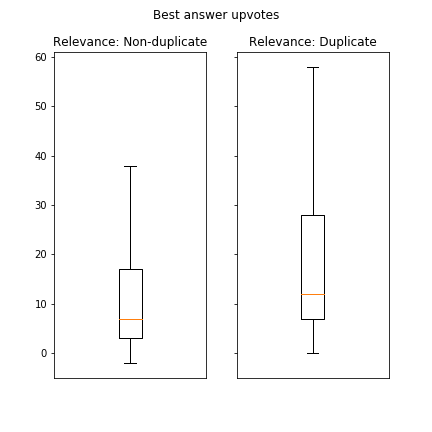
\includegraphics[width=\linewidth]{e_en_train_best_answer_upvotes.png}
        \caption{Liczba głosów na najlepszą odpowiedź.}
    \end{subfigure}
    \caption{Miary podobieństwa dla podzadania E.}
    \label{fig:e_multifigure}
\end{figure}

Powyższe wykresy (rysunki~\ref{fig:e_multifigure}) przedstawiają porównania miar statystycznych dla dwóch klas. Tak jak i w przypadku różnic długości tekstów, podobieństwa kosinusowego oraz indeksu Jaccarda, żadna z tych miar nie jest w stanie ocenić podobieństwa między dwoma tekstami.

\subsection{Sieci neuronowe}
\subsubsection{Przygotowanie danych}
Do wytrenowania sieci neuronowej wykorzystany został zbiór danych o rozkładzie przedstawionym w tablicy~\ref{se_train_set_modified}. Zbiór został podzielony na część treningową, z \emph{25407 parami tekstów}, oraz walidacyjną z \emph{5000}. Na potrzeby sieci neuronowej, etykiecie ,,Duplicate'' została przypisana wartość \emph{1}, natomiast ,,Non-duplicate'', wartość \emph{0}.

\subsubsection{Sieć syjamska}
Korzystając z eksperymentów przeprowadzonych na potrzeby poprzednich zadań, pierwszą próbą rozwiązania problemu znajdowania duplikatów za pomocą sieci neuronowych, było wykorzystanie architektury sieci syjamskich.
Architektura tej sieci została przedstawiona w rozdziale \ref{arch:malstm}. W warstwie rekurencyjnej zastosowanych zostało 50 ukrytych jednostek. Wykresy przebiegu uczenia sieci przedstawiają się następująco:

\begin{figure}[H]
\centering
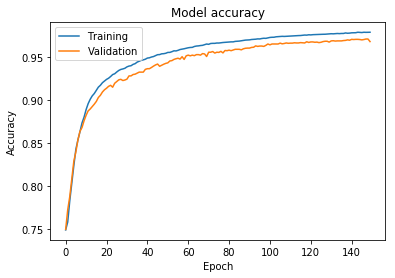
\includegraphics[scale=0.5]{e_malstm_acc.png}
\caption{Trafność sieci.}
\label{fig:e_malstm_acc}
\end{figure}

\begin{figure}[H]
\centering
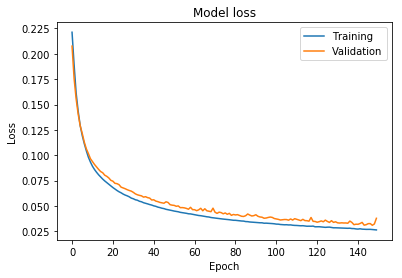
\includegraphics[scale=0.5]{e_malstm_loss.png}
\caption{Strata sieci.}
\label{fig:e_malstm_loss}
\end{figure}

Wykorzystany model sieci neuronowej sprawdził się bardzo dobrze na potrzeby tego zadania. Trafność sieci na zbiorze walidacyjnym na początku treningu wynosiła \emph{74,94\%}, natomiast po 150 epokach, wzrosła do \emph{96,84\%}. Strata w tym modelu, określona jako błąd średniokwadratowy, spadła z \emph{0,2075} do \emph{0,0308}.

\subsection{Ocena rezultatów}

Udział przeważającej klasy ,,Non-duplicate'' w zbiorze danych powoduje, że prosty klasyfikator oznaczający każdą parę zdań jako niezduplikowane miałby trafność na poziomie $\approx$~75\%. Ostateczny klasyfikator uzyskał jednak trafność $\approx$~97\%. Rozważając wyniki w oparciu o rozkład danych, można uznać, że model sieci syjamskiej potrafi z dużą dokładnością stwierdzić czy dwa teksty są swoimi duplikatami.
